\documentclass[12pt]{report}
\usepackage{amsmath}
\usepackage{graphicx}
\usepackage{caption}
\usepackage{subcaption}
 \usepackage[russian]{babel}
\usepackage{booktabs}
\usepackage{float}
\usepackage{minted}
\usepackage{verbatim}
\usepackage[utf8]{inputenc}
\usepackage{geometry}
\usepackage{multirow}
\usepackage{setspace}
\usepackage{parskip}
\usepackage[bottom]{footmisc}
\usepackage{tikz}
\usepackage[section]{placeins}

% This style is used to create block diagrams, you'll find it useful since many of your figures would be of that form, I'll try add more styles in the future :)
\usetikzlibrary{trees,positioning,fit,calc}
\tikzset{block/.style = {draw, fill=blue!20, rectangle,
                         minimum height=3em, minimum width=4em},
        input/.style = {coordinate},
        output/.style = {coordinate}
}

\usepackage[section]{minted}
\usepackage{xcolor}
\usemintedstyle{porland}

\usepackage{chngcntr}
\counterwithin{figure}{section}

\renewcommand{\arraystretch}{1.5}

\usepackage[hidelinks]{hyperref}
\hypersetup{
    linktoc=all
}

\renewcommand\listingscaption{Listing}
\renewcommand\listoflistingscaption{List of Listings}

\usepackage{scrhack}
\usepackage{tocbasic}
\setuptoc{lol}{levelup}

\usepackage{indentfirst}
\geometry{a4paper, margin=1in}

%----------EDIT COVER INFO HERE -----------------%

\def \LOGOPATH {assets/logo3.png}
\def \DEPARTEMENT {Министерство образования и науки Российской Федерации 
Федеральное государственное образовательное учреждение высшего образования
\\ «Национальный исследовательский университет «МЭИ» 
Институт ИВТ
Кафедра ПМИИ
}
\def \REPORTTITLE {Отчет по лпбораторной работе номер 3 \\ Проведение лексического анализа восходящим методом}
\def \STUDENTNAME {Желтиков Александр Алексеевич}
\def \STUDENTID {STUDNUM}


%------------------------------------------------%

\setlength{\parindent}{2em}
\setlength{\parskip}{0em}

\begin{document}

\pagenumbering{arabic}

\begin{titlepage}
    \vfill
    \begin{center}
        \includegraphics[width=0.7\textwidth]{\LOGOPATH} \\
        \hfill \\
        \Large{\DEPARTEMENT} \\
        \vfill
        \textbf{\LARGE{\REPORTTITLE}}
    \end{center}
    \vfill
    \begin{flushleft}
        \Large{\textbf{Подгтовил:} \STUDENTNAME} \\
        \Large{\textbf{Дата:} \today}
    \end{flushleft}
    \vfill
\end{titlepage}

\clearpage

\begin{center}
\Large{\textbf{1. Постановка задачи и ее условие.}}
\end{center}

\begin{flushleft}
    \text{}\newline 
    \textit{\textbf{Задание.}} С использованием лексического анализатора  lex разработать и реализовать программу восходящего лексического анализа. \\
    \text{}\newline
    \textbf{Номер варианта по журналу --> 10} \\
    \text{}\newline
    Задания предусматривают \textit{\textbf{возможность наличия комментариев неограниченной длины}} во входном языке. Форма организации комментариев соответствует языку Паскаль.\\
    Входной язык содержит операторы цикла типа \textbf{for (…; …; …) do}, разделенные символом \textbf{;} (точка с запятой). Операторы цикла содержат идентификаторы, знаки сравнения \textbf{<, >, =,} римские числа, знак присваивания \textbf{(:=)}.
\end{flushleft}
\begin{center}
\Large{\textbf{2. Грамматика лексем входного языка в форме БНФ.}}
\end{center}

\text{}\newline
<lang>::=<loop\_operator> ; <lang> | <comment> <lang> |  $\lambda$ \\
<comment>::= //[\^ \space $\backslash$n ] | "\{" \space [ \^ \space]\space "\}" \\
<loop\_operator> ::= for \textbf{"("} <assign>\textbf{";"} <compare>\textbf{";"}  <step> \textbf{")"} do  \\
<id>::= <letter> | <letter><number><id> | <letter><id>\\
<assign>::=<id>:=<expression>\\
<expression>::= <value> | <id>\\
<value>::=<number>\\
<compare>::=<id><operator> | <id> \\
<operator>::= < | > | = | <= | >=\\
<step>::= <roman> | <number>\\
<letter> ::= a | b | c | ... | z | A | B | C | ... | Z \\
<roman> ::= I | X | V \\
<number> ::= <roman> | <roman><number> \\

\begin{center}
\Large{\textbf{3. ДКА, распознающий грамматику.}}
\end{center}
\begin{center}
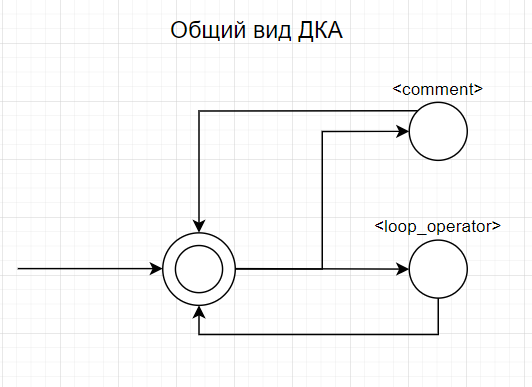
\includegraphics[width=0.7\textwidth]{assets/image.png}
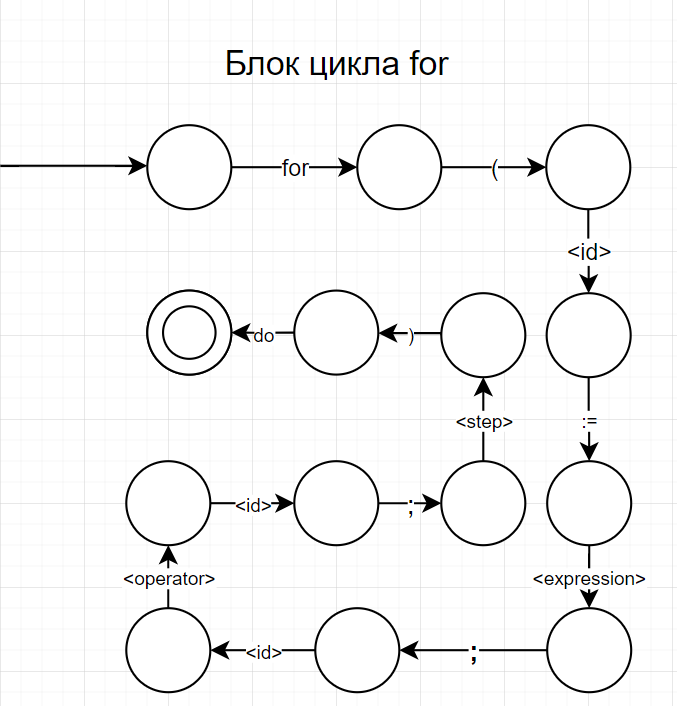
\includegraphics[width=0.7\textwidth]{assets/for.png}
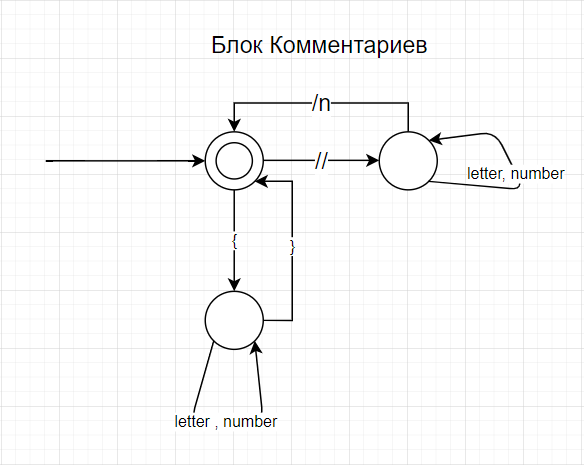
\includegraphics[width=0.7\textwidth]{assets/comment.png}
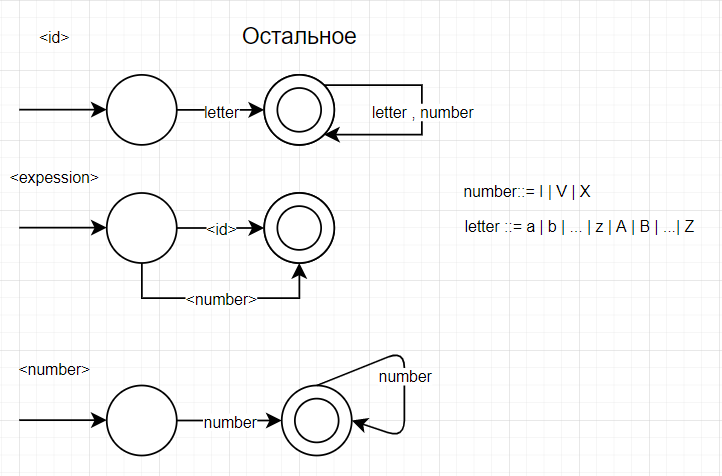
\includegraphics[width=0.7\textwidth]{assets/Other.png}
\end{center}

\begin{center}
\Large{\textbf{4. Разработка алгоритма синтаксического анализа.}}
\end{center}
\text{}\newline

Flex (Fast Lexical Analyzer) — генератор лексических анализаторов. Заменяет Lex в системах на базе пакетов GNU и имеет аналогичную функциональность. При этом Flex не является частью проекта GNU

Lex — это инструмент для лексического анализа, который может использоваться для выделения из исходного текста определенных строк заранее заданным способом. Yacc — это инструмент для грамматического разбора; он читает текст и может использоваться для конвертирования последовательности слов в структурированный формат для дальнейшей обработки.

На входе программа получает текст в свободном формате и правила выделения лексем, а на выходе даёт код анализатора, в виде функции на языке Си.[9]

Правила задаются в виде регулярных выражений слева и, обычно, кода на языке Си справа. Они содержат три секции, отделяющиеся строкой «\%\%»:
\text{}\newline \\
Блок определений \\
\%\% \\
Блок правил \\
\%\% \\
Блок кода на Си \\

Определения содержат стартовые значения и определения, правила, непосредственно сами выражения и соответствующие им действия; пользовательский код просто включается в вывод flex. Некоторые секции могут отсутствовать.

Функция анализатора получает текст на входе и выполняет заданный код для каждой найденной лексемы.

Что бы воспользоваться данным средством нужно отдельно установить его для Windows или через терминал на Linux с помощью команды. Далее (Будет использоваться система windoows 10.0) после написания кода в файле с расширением .l нужно с пощью терминала собрать полученную программу, для этого используем команду flex *.l , после компелируем полученный C-файл командой gcc lex.yy.c *.exe (где * любое имя .exe файла). В итоге, мы получаем .exe файл, который мы можем вызвать через консоль.

\begin{center}
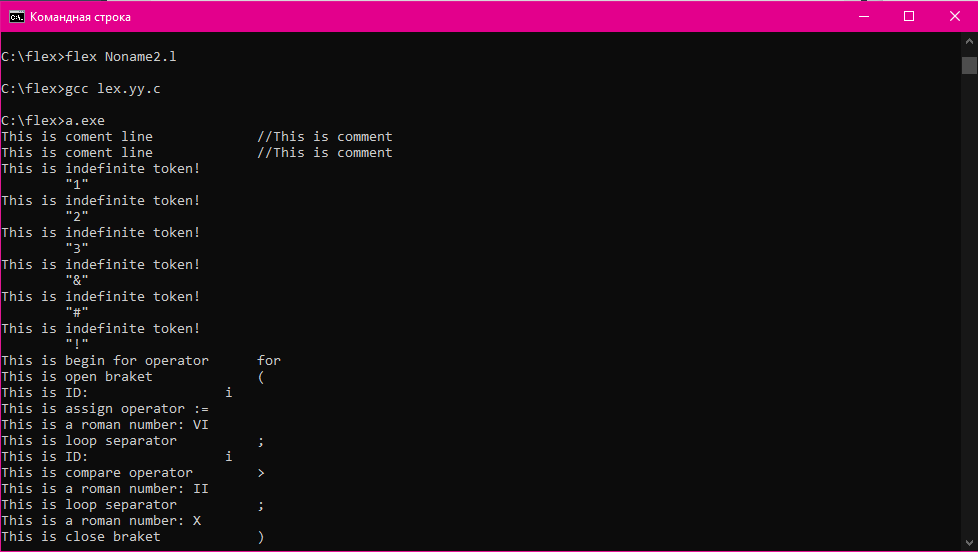
\includegraphics[width=0.7\textwidth]{assets/cmd.png}
\end{center}

\begin{center}
\Large{\textbf{5. Тестирование работы алгоритма.}}
\end{center}

Протестируем работу лексического анализатора\\
\hline 
\begin{center}
Тест номер 1:
\end{center}
\begin{minted}[fontsize=\footnotesize]{Pascal}
//This is comment
{This is 
	Multi line
	comment}
for(i := I ; i < V ; XV ) do
123 //indefinite token!
\end{minted}
\text{}\newline
\begin{center}
    Результат:\\
\end{center}
This is coment line             //This is comment\\
This is coment line             \{This is\\
        Multi line\\
        comment\}\\
This is begin for operator      for\\
This is open braket             (\\
This is ID:                 i\\
This is assign operator :=\\
This is a roman number: I\\
This is loop separator          ;\\
This is ID:                 i\\
This is compare operator        <\\
This is a roman number: V\\
This is loop separator          ;\\
This is a roman number: XV\\
This is close braket            )\\
This is end for operator        do\\
This is indefinite token!\\
        "1"\\
This is indefinite token!\\
        "2"\\
This is indefinite token!\\
        "3"\\
This is coment line             //indefinite token!\\

\hline 

\begin{center}
Тест номер 2:
\end{center}
\begin{minted}[fontsize=\footnotesize]{Pascal}
//This is comment
//This is comment
123 &#!
for(i := VI ; i > II ; X) do
\end{minted}
\text{}\newline
\begin{center}
    Результат:\\
\end{center}
This is coment line             //This is comment \\
This is coment line             //This is comment \\
This is indefinite token!\\
        "1"\\
This is indefinite token!\\
        "2"\\
This is indefinite token!\\
        "3"\\
This is indefinite token!\\
        "&"\\
This is indefinite token!\\
        "#"\\
This is indefinite token!\\
        "!"\\
This is begin for operator      for\\
This is open braket             (\\
This is ID:                 i\\
This is assign operator :=\\
This is a roman number: VI\\
This is loop separator          ;\\
This is ID:                 i\\
This is compare operator        >\\
This is a roman number: II\\
This is loop separator          ;\\
This is a roman number: X\\
This is close braket            )\\
This is end for operator        do\\
\hline 
\begin{center}
\Large{\textbf{6. Разработанный код}}
\end{center}

\begin{minted}[fontsize=\footnotesize]{c}
%option noyywrap
%{
	#include<stdio.h>
%}
FORBRA "for"
FORKET "do"
LETTER [_a-zA-Z]
NUMBER [IVX]+
MOREID {LETTER}|{NUMBER}
ID {LETTER}{MOREID}*
OPERATOR "<"|">"|"="
ASSIGN ":="
BRA "("
KET ")"
COMMENT "//"[^\n]*|"{"[^}]*"}"
SEPARATOR ";"
%%

[ \t\n]     
{FORBRA}	{printf("This is begin for operator	%s\n", yytext ); }
{FORKET}	{printf("This is end for operator	%s\n", yytext ); }
{NUMBER}	{printf("This is a roman number:	%s\n", yytext ); }
{ID}	    {printf("This is ID:	            %s\n", yytext ); }
{OPERATOR}      {printf("This is compare operator	%s\n", yytext ); }
{ASSIGN}        {printf("This is assign operator	%s\n", yytext ); }
{BRA}	   {printf("This is open braket		%s\n", yytext ); }
{KET}	   {printf("This is close braket		%s\n", yytext ); }
{COMMENT}       {printf("This is coment line		%s\n", yytext ); }
{SEPARATOR}     {printf("This is loop separator		%s\n", yytext ); }
.               {printf("This is indefinite token! \n\t\"%s\"\n", yytext );}
%%

int main()
{
	yyin = fopen( "test.txt", "r" );
	yylex();

	return 0;
}

\end{minted}

\end{document}

